%\documentclass[a4paper]{article}
\documentclass{article}
%\documentclass[journal]{IEEEtran}
%\documentclass{report}
%\documentclass{ActaOulu}

\usepackage{graphicx}
\usepackage{multirow}
\usepackage{authblk}
\usepackage{float}
\usepackage{rotating}
\usepackage{url}
\usepackage{lscape}
\usepackage{longtable}
\usepackage{subfig}
\usepackage{natbib}
\usepackage{lineno}
\usepackage{amsmath}
\usepackage{epsfig}
\usepackage{caption}
\usepackage{latexsym}
\usepackage[a4paper]{geometry}
%\setlength{\captionmargin}{20pt}
%\usepackage{graphicx}
%\usepackage[all,knot]{xy}
%\xyoption{arc}
%\usepackage{url}
%\usepackage{multimedia}
%\usepackage{hyperref}
%\linespread{1.6}
\linespread{1.2}

\newcommand{\Deg}{$^{\circ}$}
\newcommand{\Pic}[2][0.85]{\begin{center}\includegraphics[width=0.8\textwidth,height=#1\textheight,keepaspectratio]{#2}
 \end{center} }
%\newcommand{\captionfonts}{\small}
%%%%%%%%%%%%%%%%%%%%%%%%%%
% Different font in captions
\newcommand{\captionfonts}{\small}

\makeatletter  % Allow the use of @ in command names
\long\def\@makecaption#1#2{%
 \vskip\abovecaptionskip
 \sbox\@tempboxa{{\captionfonts #1: #2}}%
 \ifdim \wd\@tempboxa >\hsize
   {\captionfonts #1: #2\par}
 \else
   \hbox to\hsize{\hfil\box\@tempboxa\hfil}%
 \fi
 \vskip\belowcaptionskip}
\makeatother   % Cancel the effect of \makeatletter
%%%%%%%%%%%%%%%%%%%%%%%%%%%%
\begin{document}

\title{Numerical implementation of a sparse grid for a hyperbolic geophysical mass flow model}
\author[1]{ E. R. Stefanescu }
\author[1]{A.K. Patra}
\author[2]{K.R. Dalbey}
\author[3]{M. Bursik}
\affil[1]{Department of Mechanical and Aerospace Engineering, University at Buffalo}
\affil[2]{Sandia National Labs, Albuquerque}
\affil[3]{Department of Geology, University at Buffalo}


%\date{\today}


\maketitle

\begin{abstract}
To come soon...
\end{abstract}


\section{Introduction}
This paper describes the development of sparse grid based methodology for the propagation of input 
parameter uncertainties through a shallow-water like hyperbolic system model of 
geophysical mass flows. We apply the sparse grid based 
methodology first to the straightforward analysis of  UQ in the output of 
the model and then to the more complex construction of hazard maps based on the 
outcomes of ensembles of model runs. The results are interesting in that they show that the sparse grid 
method is quite successful in the first type of analysis where the uncertainty in a number of flow outcomes are successfully 
captured but the results from the hazard map construction that requires a more extensive exploration of the 
full parameter space to construct a response surface is not as successful.

\subsection{Background} 
\subsubsection{Need} In geophysical mass flow problems (e.g. landslides, volcanic debris flows called lahars), many flow characteristics like
material properties, the size and location of failing mass, the terrain over which the 
flow occurs at every point in the domain are difficult if not impossible to characterize. There is also much that is unknown about the
exact physics. Thus, useful outputs from the model equations governing mass flow must account for 
the variable or poorly characterized aspects of the model as well as the uncertainty of the 
parameters used in the equations \citep{Keith}. 
Most of the numerical models of real-world systems are characterized by large number of input
variables. In this case, to obtain a reliable numerical 
solution, one has to include uncertainty quantification due to the uncertainty in the input data (babuska). Furthermore, 
in many use situations of geophysical mass flows, one is concerned with flow over an entire jurisdiction (hazard analysis). 
This introduces additional complexity in the propagation of the uncertainty.

\subsubsection{Uncertainty Quantification Methods} Quantification of uncertainty means to be in some way able to attach a measure
to something which may be poorly defined or vague \citep{Matthies2008} -- in this case the outcomes of models 
with uncertain inputs. 
To quantify the uncertainties in the result of a simulation, one must understand 
both the sources of these uncertainties, and how uncertainties propagate through the simulation. 
%The recent literature on such uncertainty propagation is extensive \cite{revpap1,revpap2}.
% is there has been intensively studied the impact of errors, or uncertainty ,
%in ``data" such as parameter values, initial and boundary conditions. It came an important issue
%due to mathematical models that serve as simplified and reduced representations of the true physics.
Uncertainty quantification thus involves two steps: determination of the uncertainty sources, and 
analysis of their propagation through the simulation. In the past few years there have been 
extensive studies in the propagation of uncertainty. The common stochastic methods can be
categorized in sampling and non-sampling methods (cfdsppitt). Widely used sampling methods
are: Monte-Carlo(MC), quasi-Monte Carlo (QMC), Latin Hypercube sampling (LHS), while as 
non-sampling methods intensively used are:  Polynomial Chaos Expansion (PCE), Stochastic Galerkin (SG),
Non-Intrusive Spectral Projection (NISP), Polynomial Chaos Quadrature (PCQ) etc. 

MC methods have been applied to many applications and their implementation is straightforward.
Although the convergence rate is relatively slow, it is independent of the dimensionality of the random space and
independent of the number of random variables used to characterized the random inputs (xiuhesthaven). 
To accelerate convergence in MC, several techniques have been developed as LHS and QMC.
The PCE method uses the Wiener-Askey scheme, in which Hermite, Legendre, Laguerre, Jacobi, and generalized Laguerre
orthogonal polynomials are used for modeling the effect of uncertain variable described by normal, uniform, exponential, beta, 
and gamma distributions, respectively (eldredSandia and Xiu). These orthogonal polynomial selections are optimal for these
distribution type since the inner product weighting function and its corresponding support range correspond to the probability density 
functions for these continuous distributions. 
PCQ is a based on the PCE in general and on SG in particular. The main idea is that in addition to 
calculating the coefficients in the expansion of chaos polynomials, PCQ achieves a more accurate computation of statistical 
moments when the governing system of equations is non-polynomial, by calculating the moments directly rather than
through the intermediate coefficients.
These concepts has been used successfully in many engineering approaches over the past two decades. 
%In most of the cases it involves generation of samples of input parameter followed by the application of the
%simulation model to generate the corresponding set of stochastic responses. 
All methods have positive and negative features, and no single technique is optimum for all situations.

Recently, a stochastic collocation scheme has been introduced in which simulations are performed
at specific collocation points in the stochastic space (citation). Stochastic collocation methods for 
sPDEs have been first proposed in [XiuHesthaven and Babuska]by using numerical quadrature 
for the approximate evaluation of the stochastic integrals. 
These technique combine the exponential convergence rate of the PCE scheme with the
decoupled nature of MC techniques (sandiego). The selection of computational nodes is 
the key ingredient in all stochastic colocation methods. Choices of collocation points include
tensor product of zeros of orthogonal polynomials (citation), sparse grid (SP) methods (citation),
and probabilistic collocation(cfdsppitt).


This paper presents an approach to characterize the effect of the input uncertainty on the output 
of a geophysical mass flow model. We use the concept of stochastic collocation to account for 
uncertainties in a non-linear hyperbolic system of PDEs used in modeling geophysical mass 
flow. Neglecting the model uncertainty we focus on the input parameter uncertainty, modeled as 
random variables. Geological flow models are dealing with high dimensional input. There are large 
uncertainties associated with the construction of the DEMs and many other parameters that characterize 
the flow.

We first discuss sparse grid algorithms as an improvement of the MC, LHS and PCQ methods. 
The sparse grid scheme are chosen based on their efficiency which in most of the cases
results in a number reduction of collocation points needed to obtain a given level of approximation. 
Further, a stochastic space is defined for each problem depending on the uncertainty in
parameters. Computational points are identified in this stochastic space and simulations 
of the geophysical flow model are performed. Our goal is to compute the statistics of the 
output in form of mass velocity, maximum height of the pile over time, momentum etc and
compare the convergence for the above mentioned methods. 
 

Sparse grid schemes have been successfully implemented for parabolic and elliptic sPDEs.
(Borziaustria) proposed a framework combining space-time multigrid methods with sparse grid
collocation techniques to solve a nonlinear parabolic system with random coefficients, while
(Babuskanobile) proposed a stochastic collocation method to solve elliptic partial differential
equations with random coefficients and forcing terms. In the paper of (cfdspitt) a numerical 
simulations is done for an incompressible and slightly compressible single and the two-phase 
flow in porous media. The stochastic domain is represented using collocation at the zeros of 
tensor product Hermite polynomials. It was observed that the stochastic collocation converges
much faster (to the mean and variance) than the standard MC approach with a significantly 
reduced number of simulations. In the paper (Melosh07) a comparison of the accuracy and 
efficiency of the sparse grid collocation approach to MC and GPCE is performed, when used 
to solve a natural convection problem.

\subsection{Hazard Analysis} Determining the risk associated with geophysical flows has been a effort of a large scientific
community (citation). In areas of flood hazards the delineation of  regions into zones of high and low risk
is usually based on the probability of a critical threshold for some parameter associated with 
the hazard map being exceeded.
In the paper, we also propose to investigate the use of sparse grid design (SPD) for hazard 
map construction. Sparse grids provide sampling points which avoid the curse of dimensionality.
A Bayes Linear Model (BLM) is used to fit the data and construct a hazard map. 


The paper is organized as follows: we first give a brief description of the non-linear hyperbolic systems
used in modeling geophysical mass flows. Then we proceed to discuss sparse grid schemes 
in section 3 and details of numerical implementation in section 4. Finally discussions and conclusions
are presented in section 5.

\section{Basic model}
\subsection{Governing equations}
The geophysical mass flow code - TITAN2D combines numerical simulations of the flow with
digital data of the natural terrain. It is based on a depth-averaged
model for an incompressible granular material, governed by
Coulomb-type friction interactions \citep{Savage1989}.  The
governing equations are obtained by applying conservation laws to the
incompressible continuum, providing appropriate constitutive modeling
assumtions, and then taking advantage of the shallowness of the flows
(flows are much longer and wider than they are deep) to obtain simpler
depth-averaged representations \citep{Patra2005}. The motion of the
material is considered to be gravitationally driven and resisted by
both internal and bed friction forces. The stress boundary conditions
are: no stress at the upper free-surface and a Coulomb-like friction law
imposed at the interface between the material and the basal
surface. The resulting hyperbolic system of equations is solved using a
finite-volume scheme -- with a second-order -- Godunov solver. Even if many
real geophysical flows such as debris flow are fluidized, in this
study we deal only with granular material that has not been fluidized.

\begin{align} \nonumber
&\frac{\partial{h}}{\partial{t}} + \frac{\partial{(V_x \cdot h)}}{\partial{x}} + \frac{\partial{(V_y \cdot h)}}{\partial{y}} &= 0 \\ 
&\frac{\partial{hV_x}}{\partial{t}} + \frac{\partial{(V_x \cdot hV_x + 0.5 k_{ap}g_zh^2)}}{\partial{x}} + \frac{\partial{(V_y \cdot hV_x)}}{\partial{y}} &={S_x} \\  \nonumber
&\frac{\partial{hV_y}}{\partial{t}} + \frac{\partial{(V_x \cdot hV_y)}}{\partial{x}} + \frac{\partial{(V_y \cdot hV_y + 0.5 k_{ap}g_zh^2)}}{\partial{y}} &= S_y \\ \nonumber
\label{eqn1}
\end{align}
where 
\begin{align} \nonumber
&k_{ap} = 2\frac{1\mp \sqrt{1-cos^2(\phi_{int})(1+\tan^2(\phi_{bed}))}}{\cos^2} -  1  \\ \nonumber
\end{align}
The source terms are defined as:
\begin{align} 
&S_x = g_xh -\frac{V_x}{\sqrt{V_x^2+V_y^2}}\max{\left(g_z + \frac{V_x^2}{r_x}, 0 \right)} h \tan((\phi_{bed}) - 
-  sgn \left( \frac{\partial{V_x}}{\partial{y}} \right )h k_{ap} \frac{\partial{(g_xh)}}{\partial{y}} \sin((\phi_{int}) \\
&S_y = g_yh -\frac{V_y}{\sqrt{V_x^2+V_y^2}}\max{\left(g_z + \frac{V_y^2}{r_y}, 0 \right)} h \tan((\phi_{bed}) -  \nonumber
-  sgn \left( \frac{\partial{V_y}}{\partial{x}} \right )h k_{ap} \frac{\partial{(g_yh)}}{\partial{x}} \sin((\phi_{int}) \\  \nonumber
\end{align}

where, $h$ is the height of the flow, $hV_x, hV_y$ are moments in $x$ and $y$ directions, $g = \{g_x,g_y,g_z\}$ are
components of the gravity along the three axes. $\phi_{int}$ and $\phi_{bed}$ are the internal and basal friction angles,
respectively, and $r_x$ and $r_y$ are the radii of curvature of terrain in the $x$ and $y$ directions.

\subsection{Parameters uncertainty}
TITAN2D was developed for modeling dry geophysical granular flows,
such as debris avalanches and block and ash flows.  Given a digital
elevation map specifying the topography of a volcano and the values of
input parameters, including the initial volume of erupted material and
the friction angles, TITAN2D calculates the flow depth and velocity at
any location throughout the duration of an event. There is uncertainty 
in all of the input parameters. It was found by (Keith) that the flow is fairly
insensitive to internal friction angle, but bed friction angle and the size of the
initial flowing mass are important. The degree of sensitivity to initial location
highly depends on the local terrain features in the neighborhood of the
starting location. The combination of uncertainty and sensitivity to these
inputs dictates which ones need to be represented as random variables.
 
\section{Stochastic numeric methods}
To account for the impact of the uncertainty in the parameters, it is natural to consider moments
of the solutions over the probabilistic space. In other words, we need to evaluate multi-dimensional
integrals (Gaobrowndiffeqn). The main idea of the stochastic collocation approach is to abandon the 
random sampling approach and consider the use of the more advanced integration approaches as 
hierarchical integration techniques.

We are interested in convergence of the first and second moment of the model output when using sparse
grid as a colocation method. In an attempt to minimize the number of sample points we use sparse grid
schemes. The colocation points in the high-dimensional random parameters space is significantly reduced 
compared to a full tensor product. 

The MC, LHS, PCQ and SP approaches follow identical procedures except in the 
choice of grid points in the sample space and the quadrature weights associated with those 
points. These procedures and the choices of collocation points for the SP are described below.

\subsection{Monte Carlo simulations}
In a typical MC simulation with $N_{MC}$ number of samples the mean converges asymptotically as 
$\sqrt{N_{MC}^{-1}}$, and is independent of the number of random dimensions, $N$ (linpacificlab).
The general procedure for MC simulation of transport equations is:
\begin{itemize}
\item Generate $N_{MC}$ sample
\item Solve the deterministic problem for each sample
\item Stochastic moments are computed as simple arithmetic means
\begin{equation}
\langle U(\xi_{i=1\cdots N_{MC}})^N\rangle = \frac{1}{N_{MC}}\sum_{i=1}^{N_{MC}}U(\xi_i)^N
\end{equation}
The mean is given as mean(U) = $\langle$ U $\rangle$. By the central limit theorem (Chung, and more)
the accuracy is $\frac{\sigma}{\sqrt{N_{MC}}}$, where $\sigma$ is the standard deviation of the estimate. 
Thus to double the accuracy, it is necessary to quadruple the number of sample points (keithpaper). 
\end{itemize}

\subsection{Latin Hypercube Sampling}
The Latin Hypercube Sampling is implemented as bellow:
\begin{itemize}
\item For each random dimension/variable generate $N_{pts}$, using a method improved by (keithpaper)
\item For every $i=1,\cdots,N_{pts}$ points, one value from each of the $N_{dir}$ random direction is taken
to form the coordinates of the point in the $N_{dir}$-dimensional sample space.
\item Evaluate the model for this value of the sample space.
\item Expectations and other statistics are calculated as in MC. 
\end{itemize}

\subsection{PCQ}
PCQ is natural evolution of the SG, only that the evaluation of the projections is performed 
through quadrature - that is, via numerical rather than analytical integration. 
It leads to a method that has the simplicity of MC and cost of PC. A detailed explanation
can be found in (keithpaper).

\subsection{Sparse grid collocation method}
%Means, variances, and higher moments of random variables are integrals. These integrals must be
%computed numerically for large-scale systems, and thus, because of the ``curse of dimensionality",
%become problems of efficiently sampling a multi-dimensional random space (mitsppdf). Numerical
%integration is a problem of efficiently characterizing a function over a space by sampling it at discrete
%points: $\int f(x) dx \approx \sum_i w_if(x_i)$. 
\subsubsection{One dimension}
%To find an approximate solution, one possible approach is Monte Carlo simulation. Other strategies
%like Riemann sums with regularly-spaced modes are also straightforward.
A general univariate integration problem can be written as :
\begin{equation}
I[g] = \int_{\Omega} g(x) w(x) dx
\end{equation}
Where $x$ represents a random variable, $g(x)$ is a function in $x$ and $w(x)$ 
represents the p.d.f. of $x$ with support $\Omega$.
The polynomial-based approaches fit polynomials to the integrand, and the resulting polynomial 
function is then integrated. In general, the nodes are the roots of the fitted polynomials.
A sequence of quadrature rule is defined $V = \{V_i : i\in N\}$ and each
 rule $V_i$ specifies a set of rule $X_i \subset R$ and a corresponding weight 
 function $w_i :X_i \longrightarrow R$ . The optimal abscissas of the
 $n-$point Gaussian quadrature formulas are the roots of an orthogonal polynomial
 for the same interval and weighting function. In this case the approximation of $I$ by $V_i$ 
 is given as : 
\begin{equation}
V_i[g] =\sum_{x \in X_i}g(x) w_i(x) dx
\end{equation}

\textbf{Gauss-Legendre } \\ 
Gaussian quadrature is the best known polynomial-based method, famed for its $2n-1$ degree of 
polynomial exactness, meaning that with $n$ function evaluations, all integrands which are 
polynomials of order $2n -1$ or less will be integrated exactly. Gaussian quadrature utilizes 
orthogonal polynomials, such as Legendre, Hermite, or Laguerre polynomials. When approximating
expectations of functions of random variable, the choice of orthogonal polynomial should reflect the
type of random variable. Legendre polynomials should be used for uniform random variables, and 
Hermite polynomials for normal random variables. However, the Gauss-Legendre formulas are in
general not nested.\\

\textbf{Gauss-Kronrod-Patterson quadrature rules}\\
Gauss-Kronrod-Patterson (citation) quadrature are an extension of Gaussian rules first developed by
Kronrod and then iterated by Patterson to yield a sequence of nested quadratures: the set of
nodes for each level are contained in the nodes for all successive levels. In the sparse grid 
formulation nesting allows function evaluations to be reused. 
Thus, the $n$-point Gauss quadrature formula was extended by $n+1$ points (zeros of the Stieltjes
polynomials such that the polynomials) degree of exactness or the resulting $2n+1$ formula is maximal.\\

\textbf{Clenshaw-Curtis}\\
The nodes of Clenshaw-Curtis (citation) quadrature are at the roots of Chebyshev polynomials and
is exact for polynomial of order n when $n+1$ points are used.
For a given level $k \in N$ the sequence of $n_l$-point quadrature formula is:
\begin{equation}
n_k= \left \{ \begin{array}{ll}
                    2^{k-1} + 1 & \mbox{if $k>1$}\\
                    1 &\mbox{if $k=1$}
              \end{array}
              \right.
\end{equation}
And the abscissas are given by:
\begin{equation}
x_{ki}= \left \{ \begin{array}{ll}
                   -\frac{1}{2}\cdot(\cos\frac{\pi \cdot (i-1)}{n_k-1}+1) & \mbox{for $k=1,\cdots,n_k$, if $n_k >1$}\\
                    1 &\mbox{for $k=1$, if $n_k=1$}
              \end{array}
              \right.
\end{equation}

When considering the efficiency of the integration measured through polynomial exactness, it is
worth keeping in mind that polynomial exactness is just one measure of accuracy and making
other choices may well better highlight the advantages of other methods. It was shown by (Threfethen 
and Gaobrown) that the Clenshaw-Curtis very often is comparable or even better in accuracy to Gauss
quadrature despite formally having lower polynomial exactness. This behavior will be observed 
in section 4 in the construction of the hazard map.

\subsubsection{Multiple dimensions}
The extension of the univariate quadrature rules to multiple dimensions can be achieved by 
the product rule. 

\textbf{Full Grids}\\
 The use of a full tensor product space is attractive in the case of a small number of random variables.
 In D dimensions, the number of evaluations of the function grows exponentially and as dimension
 grows, the error order grows as well at an exponential rate: $\mathcal{O}(n_{q}^{-r/D})$.
 This is defined for functions in $C^r$ (function with bounded mixed derivatives up to order r)
 and where $n_q$ is the total number if points in the grid.
 If the number of random variables is moderate or large, one should rather consider full polynomial 
 space or sparse tensor product spaces. 

 \textbf{Sparse Grids}\\
 Smolyak (1963) introduced what is now known as Smolyak's formula and is the underlying formulation
 of all sparse grid methods (MITsp and more). Define the level $i$ difference quadrature:
 \begin{equation}
\Delta_i = V_i - V_{i-1},  \; V_0 = 0 \; \forall i \in N
\end{equation}
With $\textbf{i} = [i_1, \cdots, i_D]$, define for any $q \in N_0$:
 \begin{equation}
N_q^D = \lbrace \textbf{i} \in N^D : \sum_{d=1}^{D} i_d=D + q \rbrace 
\end{equation}
and $N_{q}^D = \emptyset$ for $q \le 0$. \\
 The Smolyak rule with accuracy level $k \in N$ for D-dimensions:
 \begin{equation}
A_{D,k}[g] = \sum_{q=0}^{k-1}\sum_{\textbf{i}\in N_{q}^D} (\Delta_{i_1} \otimes \cdots \otimes \Delta_{i_D})[g]
\end{equation}
The above rule was improved by (Wasilowki) by expressing $A_{D,k}[g]$ directly
in terms of the univariate quadrature rules instead of their differences.
\begin{equation}
A_{D,k}[g] = \sum_{q=k-D}^{k-1}(-1)^{k-1-q}\begin{pmatrix}D-1 \\ k-1-q \end{pmatrix}
\sum_{i \in N_q^D}(V_{i_1} \otimes \cdots \otimes V_{i_D})[g]
\end{equation}
 It can be seen that nesting causes points of different grids in the sum to coincide, and the number of
 common points increases with both the level and dimension of the sparse grid (Fig.~\ref{fig1}).
 The error for a sparse grid can be estimate as:
 \begin{equation}
\lvert I[g] -A_{D,q}[g] \rvert = \mathcal{O}(n_{q}^{-r}\log(n_q)^{(D-1)(r+1)})
\end{equation}
 The advantage of the stochastic collocation approach on sparse grids with respect to, e.g., Monte Carlo 
 simulation, is to reduce the number of solver calls.
 The Smolyak algorithm provides a way to construct interpolation functions based on a minimal number
 of points in multi-dimensional space. When one is dealing with multiple stochastic dimensions, it is 
 straightforward to extend the interpolation functions in the one dimension to multiple dimensions by 
 using tensor products in this special way (hierarchicalxiangma, klimkethesis, Melosh07). The algorithm 
 provides a linear combination of tensor products chosen in such a way that the interpolation error is 
 nearly the same as the full-tensor product in higher dimensions. 
 %As the dimension of the problem increases the number of points required can be several order of
 %magnitude different. \\

\section{Numerical implementation}
Inputs to the TITAN2D code are the size and the location of the mass at 
initiation, internal and bed friction angle, and a digital elevation map (DEM)
of the topography. One of the output file produced by the code contains
the mass averaged velocity and maximum height of the pile.

As a first step of the analysis, a sparse grid implementation is used to 
propagate the input parameter uncertainties through a shallow-water 
like hyperbolic system model of geophysical mass flows. High order 
moments of the output were calculated. We are going to extend 
the work of (keith),  which illustrated the MC, LHS and 
PCQ for the granular flow equations as applied to a slumping
flow of a cylinder of granular material.  
In this paper, a comparison on the convergency of the mean and standard
deviation is performed for the case when we are dealing with 2 and 4 random 
input parameters. 

% is Sparse Grid Design for the construction of a 
%hazard map. In general volcanic hazard maps are used to portray potential
%future geological events (sheridan). When a crisis develops at a volcano a 
%fast and reliable map is needed. Uncertainties in data regarding flow
%characteristics and in the construction of the DEM complicate the construction 
%of accurate hazard maps. In previous work (Stefanescu2010), a LHS design to
%sample the input space was implemented for 4 and 8 input parameters. 

Since many of the modeling applications are characterized by 
large number of input variables, TITAN2D being also the case, we try to
explore the high-dimensional input variable space and its impact on the model.
An important concern is the number of experiment or modeling simulations 
necessary to learn the effect of the system input on the output behavior.
Full space analysis without any a priori assumption has an exponential 
growing computational complexity, which leeds to some "smart" way of sampling
the parameter space. In the paper, we implemented a Sparse Grid Design (SPD) and LHS.

The following steps were performed in the analysis:
\begin{itemize}
\item Collocation points were generated in the stochastic domain
at different level of accuracy. The sparse grid toolkit \textit{spinterp}
(citation) is employed for this purpose.
\item Weights corresponding to each collocation point are determined.
\item At each collocation point, TITAN2D simulations are performed and
the relevant outputs are stored.
\item A comparison of the outputs is done for each study case.  
\end{itemize} 

\subsection{Slumping pile - 2 RV}
We considered the case of a cylindrical pile of granular material,
with a 10 cm height and radius, resting on a horizontal surface that
is suddenly released. The bed and internal friction angles have random
distributions:
\begin{equation} 
\phi_{bed} = (20 + 5\xi_1)\frac{\pi}{180} \\
\end{equation} 
\begin{equation} \nonumber
\phi_{int} = \phi_{bed} + (5 + 3\xi_2)\frac{\pi}{180}
\end{equation} 
were $\xi_1$ and $\xi_2$ are uniform distributed between -1 and 1.
We are using a Gauss-Legendre and Kronrod-Gauss-Paterson type 
sparse grid to calculate the mean and the standard deviation of averaged velocity
and maximum pile height of the pile after 3.0 seconds. Figure ~\ref{fig2} 
and \ref{fig3} show the way the simulations points are distributed 
in the input space. 

\subsection{Slumping pile - 4 RV}
The random variables in this study case are $\phi_{bed} \sim\mathcal{U}(15-22)$,
$\phi_{int} \sim\mathcal{U}(20-34)$, and the volume of the initial pile. The shape 
of the initial failure region is approximated as a paraboloid and gives a good
approximation of the volume range. The radius values were uniformly distributed 
between 10 and 20 mm, while the initial height followed the same distribution with values 
between 10 and 20 mm. Additional to SP runs, MC, LHS and PCQ simulations were 
performed.

\subsection{Real study case}
In the next step of our analysis we applied the computational model to
a more complex scenario. In this case are dealing with the digital terrain
representation of Mammoth Mountain, which is a large, geologically 
young volcano located on the southwestern rim of the Long Valley 
Caldera, California \citep{Bailey1989}. 
Along with uncertainties in the DEM, other four 
parameters are used to set the bounds of the computational modeling:
internal friction angle, basal friction angle, volume of the flows, and location 
of the initial pile. 
Based on the knowledge acquired from the domain expert  involved in the 
analysis and previous work in hazard analysis using TITAN2D(citation), we 
chose parameters for the flow models to bracket the range of flow volumes 
and to be representative of the friction angles that have been used by other
researchers in their computational models.  
Many TITAN2D users have chosen values of internal friction that range between
15 and 37 degrees with
values between 30 and 35 being the most frequent values used
\citep{Patra2005, murcia_2010}.  For our study we use an internal
friction angle uniformly distributed between 20 and 25 degrees.
We are using a basal friction angle
uniformly distributed between 15 and 20 degrees.
Block and ash flows on Mammoth Mountain might contain $O(10^5 -
10^7) m^3$ of material \citep{Patra2005, Burkett2007}.  Thus, our
choice of volumes ranges from $1.9 \times 10^5$ to $5 \times 10^6
m^3$.  
Initiation locations were taken from previous mapping of vent sites,
coupled with knowledge of known weak areas within the volcano as
indicated by hydrothermal alteration.  Around the centers of the
separate initiation locations, different starting positions were
uniformly distributed in a circle of radius 200 m.  

??For a better understanding of the effect of the increase in dimension
of the input space simulation for 4 RV,  and 8 RV were performed.


\section{Results and Conclusions}

\begin{figure}[H]
      \begin{minipage}[b]{0.6\textwidth}
        \begin{tabular}{c}
       % \Pic[0.3]{SRTM30_dem.jpg}\\
       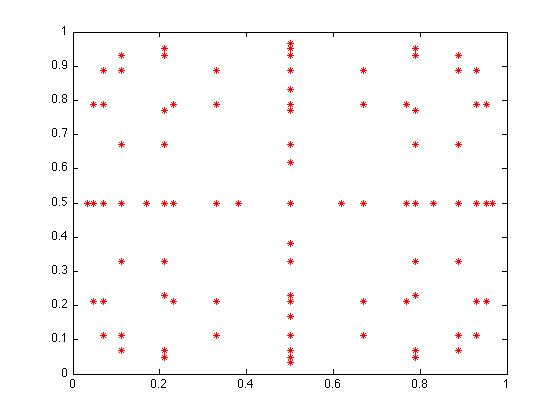
\includegraphics[width=8cm,height=9cm,keepaspectratio]{fig/GQU_2_6.jpg}\\
        (a)
        \end{tabular}
    \end{minipage}
%\hfill
    \begin{minipage}{0.6\textwidth}
        \begin{tabular}{c}
       % \Pic[0.3]{NED30_dem.jpg}\\
	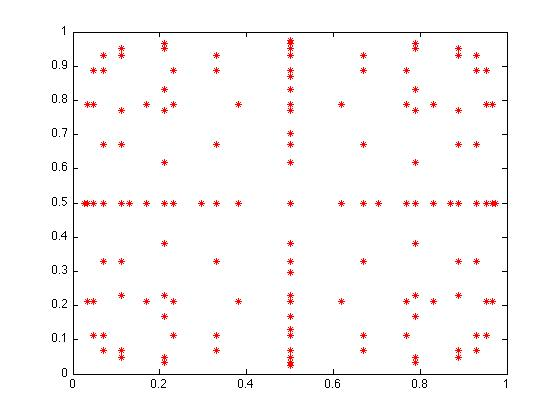
\includegraphics[width=8cm,height=9cm,keepaspectratio]{fig/GQU_2_7.jpg}\\
        (b)
        \end{tabular}
    \end{minipage} 
    \begin{minipage}[b]{0.6\textwidth}
        \begin{tabular}{c}
       % \Pic[0.3]{SRTM30_dem.jpg}\\
       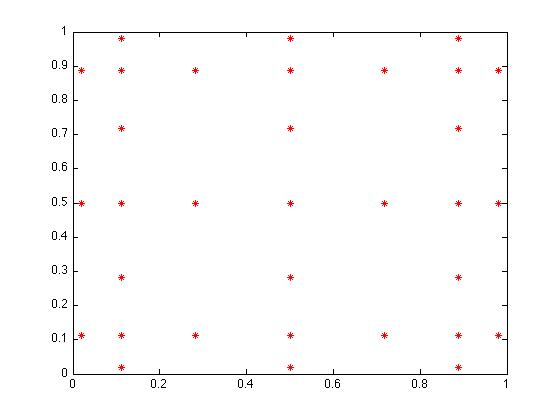
\includegraphics[width=8cm,height=9cm,keepaspectratio]{fig/KPU_2_6.jpg}\\
        (c)
        \end{tabular}
    \end{minipage}
%\hfill
    \begin{minipage}{0.6\textwidth}
        \begin{tabular}{c}
       % \Pic[0.3]{NED30_dem.jpg}\\
	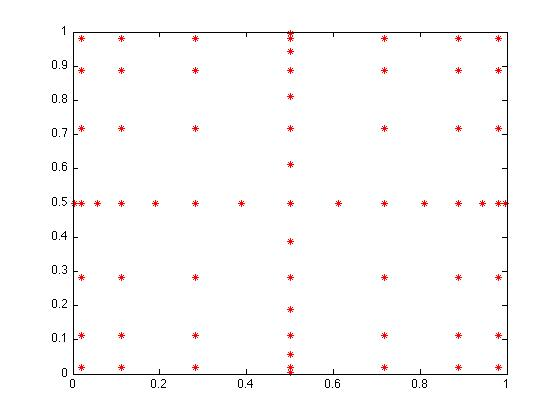
\includegraphics[width=8cm,height=9cm,keepaspectratio]{fig/KPU_2_7.jpg}\\
        (d)
        \end{tabular}
    \end{minipage} 
\caption{(a) Gauss-Legendre level 6 of accuracy
(b) Gauss-Legendre level 7 of accuracy
(c) Kronrod-Paterson level 6 of accuracy
(d) Kronrod-Paterson level 7 of accuracy }
\label{fig1}  
\end{figure}

\begin{figure}[H]
      \begin{minipage}[b]{0.6\textwidth}
        \begin{tabular}{c}
       % \Pic[0.3]{SRTM30_dem.jpg}\\
       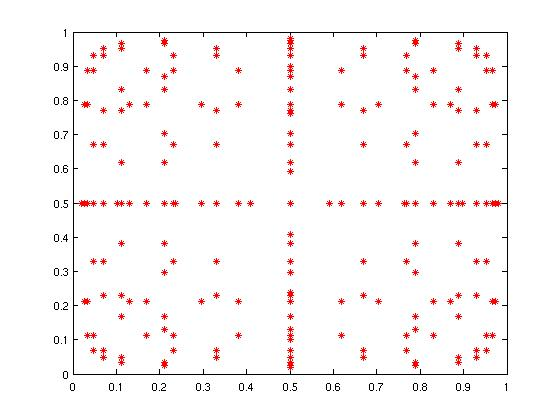
\includegraphics[width=8cm,height=9cm,keepaspectratio]{fig/GQU_a_210.jpg}\\
        (a)
        \end{tabular}
    \end{minipage}
%\hfill
    \begin{minipage}{0.6\textwidth}
        \begin{tabular}{c}
       % \Pic[0.3]{NED30_dem.jpg}\\
	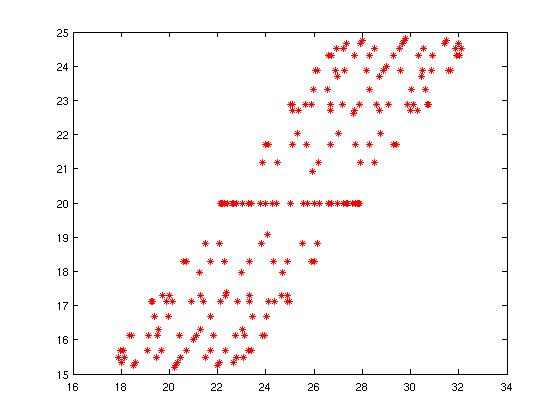
\includegraphics[width=8cm,height=9cm,keepaspectratio]{fig/GQU_b_201.jpg}\\
        (b)
        \end{tabular}
    \end{minipage} 
    \begin{minipage}[b]{0.6\textwidth}
        \begin{tabular}{c}
       % \Pic[0.3]{SRTM30_dem.jpg}\\
       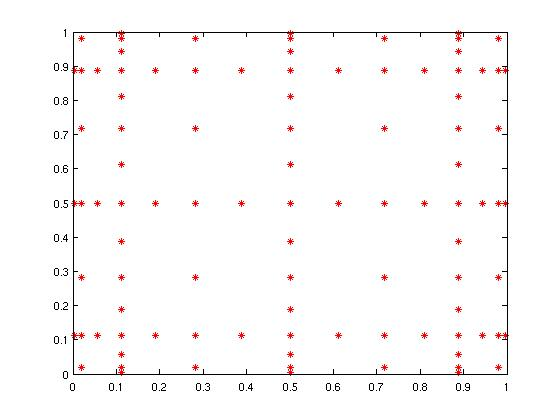
\includegraphics[width=8cm,height=9cm,keepaspectratio]{fig/KPU_a_97.jpg}\\
        (c)
        \end{tabular}
    \end{minipage}
%\hfill
    \begin{minipage}{0.6\textwidth}
        \begin{tabular}{c}
       % \Pic[0.3]{NED30_dem.jpg}\\
	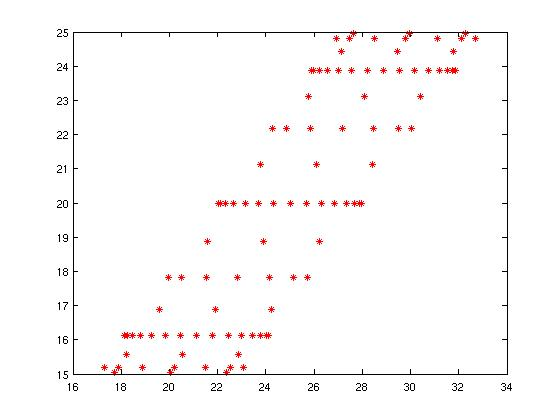
\includegraphics[width=8cm,height=9cm,keepaspectratio]{fig/KPU_b_97.jpg}\\
        (d)
        \end{tabular}
    \end{minipage} 
\caption{(a) GQU 201 grid points level 8 of accuracy (bed friction 
vs internal friction angle) b) KPU 97 grid points level 8 of accuracy
(bed friction vs internal friction angle)}
\label{fig2}  
\end{figure}

\begin{figure}[H]
      \begin{minipage}[b]{0.6\textwidth}
        \begin{tabular}{c}
       % \Pic[0.3]{SRTM30_dem.jpg}\\
       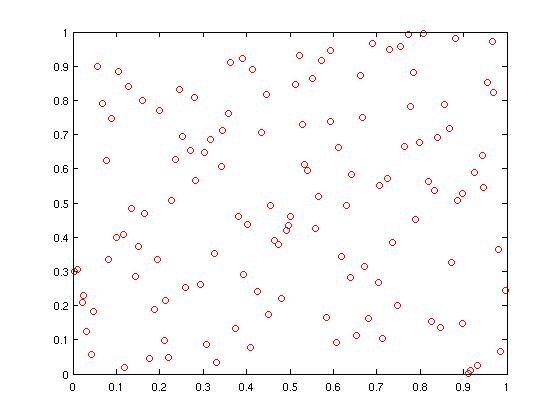
\includegraphics[width=8cm,height=9cm,keepaspectratio]{fig/lhs_b_128.jpg}\\
        (a)
        \end{tabular}
    \end{minipage}
      \begin{minipage}[b]{0.6\textwidth}
        \begin{tabular}{c}
       % \Pic[0.3]{SRTM30_dem.jpg}\\
       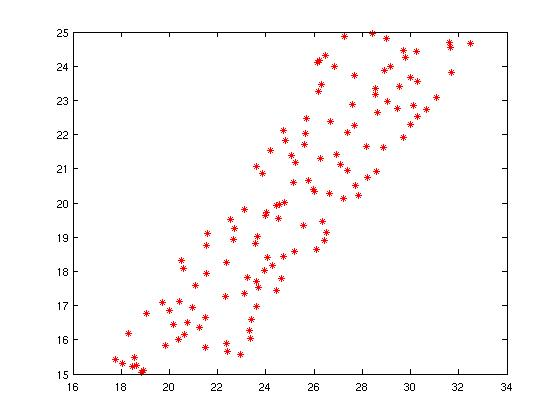
\includegraphics[width=8cm,height=9cm,keepaspectratio]{fig/lhs_a_128.jpg}\\
        (b)
        \end{tabular}
    \end{minipage}
%\hfill
    \begin{minipage}{0.6\textwidth}
        \begin{tabular}{c}
       % \Pic[0.3]{NED30_dem.jpg}\\
	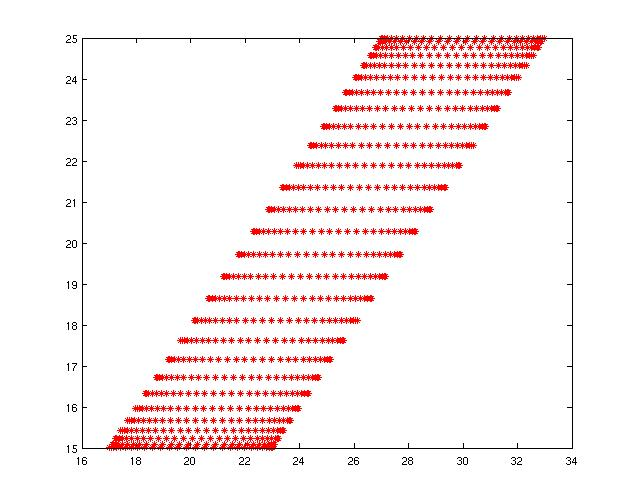
\includegraphics[width=8cm,height=9cm,keepaspectratio]{fig/PCQ_783.jpg}\\
        (c)
        \end{tabular}
    \end{minipage}
   % \begin{centering} 
   \begin{minipage}[c]{0.6\textwidth}
       \begin{tabular}{c}
       % \Pic[0.3]{SRTM30_dem.jpg}\\
       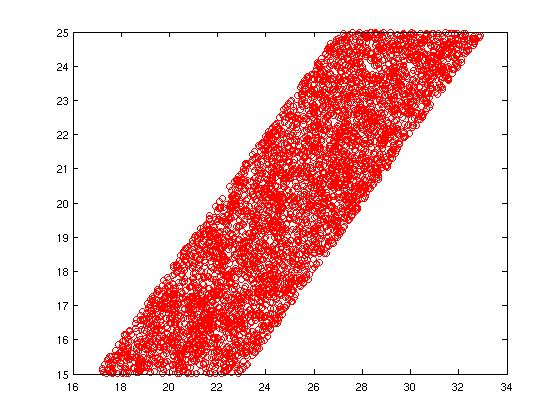
\includegraphics[width=8cm,height=9cm,keepaspectratio]{fig/mc_4444.jpg}\\
        (d)
        \end{tabular}
    \end{minipage}
    %\end{centering}
\caption{a) LHS 128 grid points (bed friction vs internal friction angle)
b) PCQ 783 grid points c) MC 4444 grid points }
\label{fig3}  
\end{figure}

\begin{figure}[H]
      \begin{minipage}[b]{0.6\textwidth}
        \begin{tabular}{c}
       % \Pic[0.3]{SRTM30_dem.jpg}\\
       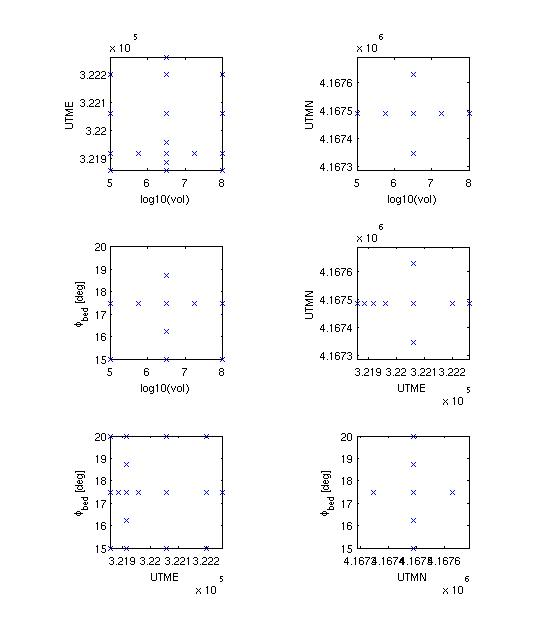
\includegraphics[width=8cm,height=9cm,keepaspectratio]{fig/picsdistrib/Clenshaw_grid.jpg}\\
        (a)
        \end{tabular}
    \end{minipage}
      \begin{minipage}[b]{0.6\textwidth}
        \begin{tabular}{c}
       % \Pic[0.3]{SRTM30_dem.jpg}\\
       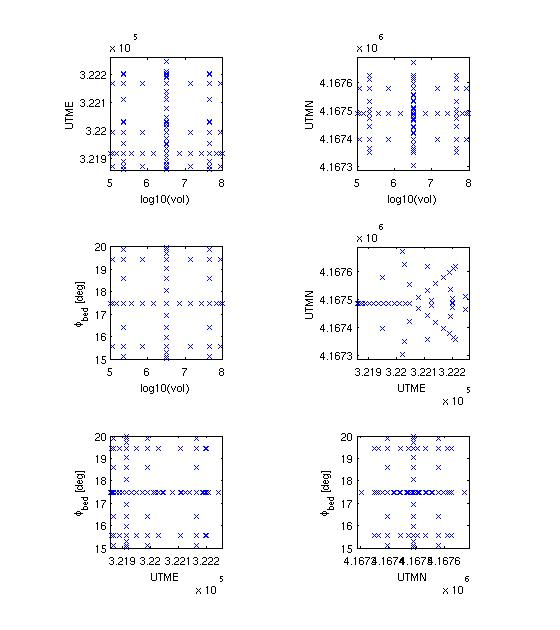
\includegraphics[width=8cm,height=9cm,keepaspectratio]{fig/picsdistrib/Clenshaw_grid_160.jpg}\\
        (b)
        \end{tabular}
    \end{minipage}
%\hfill
    \begin{minipage}{0.6\textwidth}
        \begin{tabular}{c}
       % \Pic[0.3]{NED30_dem.jpg}\\
	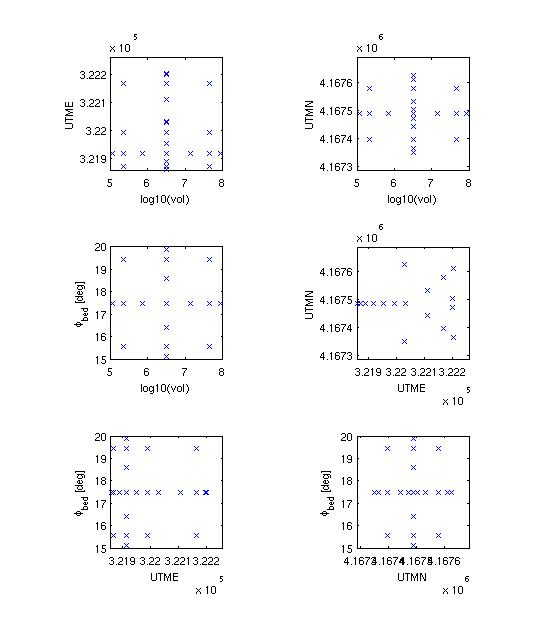
\includegraphics[width=8cm,height=9cm,keepaspectratio]{fig/picsdistrib/Gauss_Patterson.jpg}\\
        (c)
        \end{tabular}
    \end{minipage}
   % \begin{centering} 
   \begin{minipage}[c]{0.6\textwidth}
       \begin{tabular}{c}
       % \Pic[0.3]{SRTM30_dem.jpg}\\
       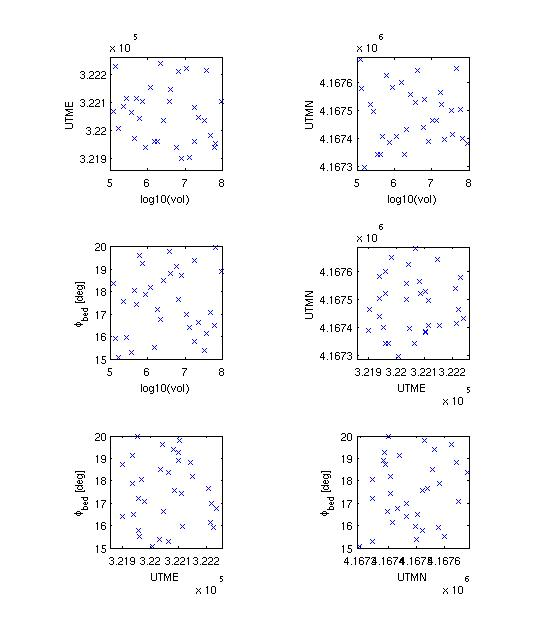
\includegraphics[width=8cm,height=9cm,keepaspectratio]{fig/picsdistrib/lhs_32.jpg}\\
        (d)
        \end{tabular}
    \end{minipage}
    %\end{centering}
\caption{ These plots are projections of a 4-dimensional random variable for a) CC - 32 sample points
b) CC - 114 sample points c) GP - 144 sample points (d) LHS -128 sample points }
\label{fig4}  
\end{figure}



\bibliographystyle{plainnat}	
%\bibliographystyle{plainyr}	
\bibliography{mybib}	
\end{document}
